\chapter{Simulation model and validation}
\label{ch:model}

\section{Model structure}

The converter is modelled in PLECS~\cite{plecs}. The model contains:
\begin{itemize}
  \item three half-bridge modules on a common heat sink;
  \item the \SI{200}{\micro\farad} DC-link with its ESR;
  \item a \SI{5}{\micro\henry} source inductance for the battery cables;
  \item an $RL$ load per phase;
  \item the modulator of \cref{ch:modulation}.
\end{itemize}
The devices use the vendor thermal description~\cite{wolfspeed_plecs}. It
gives the conduction and switching losses as tables of current, voltage and
junction temperature. It scales the switching energy with the gate
resistance. The model passes it the design values, \SI{5}{\ohm} at turn-on
and \SI{12.5}{\ohm} at turn-off.

For the \device{} the vendor gives the description in the older two-file
format (MOSFET and body diode), while the model uses the newer single-file
format. A script converts one into the other. It was tested on the
C3M0040120K, which exists in both formats: all \num{579} table values of the
conversion equal the vendor's own single file.

All simulations run from Python through the PLECS XML-RPC interface. Every
figure and number of this report can be reproduced with one command.

\section{Spectra}

PLECS uses a variable time step, so its output is not uniformly sampled. For
the spectra the solver is asked for a uniform grid that covers a whole number
of output periods. The fundamental then falls exactly on one bin and no
window is needed.

\begin{figure}[htbp]
\centering
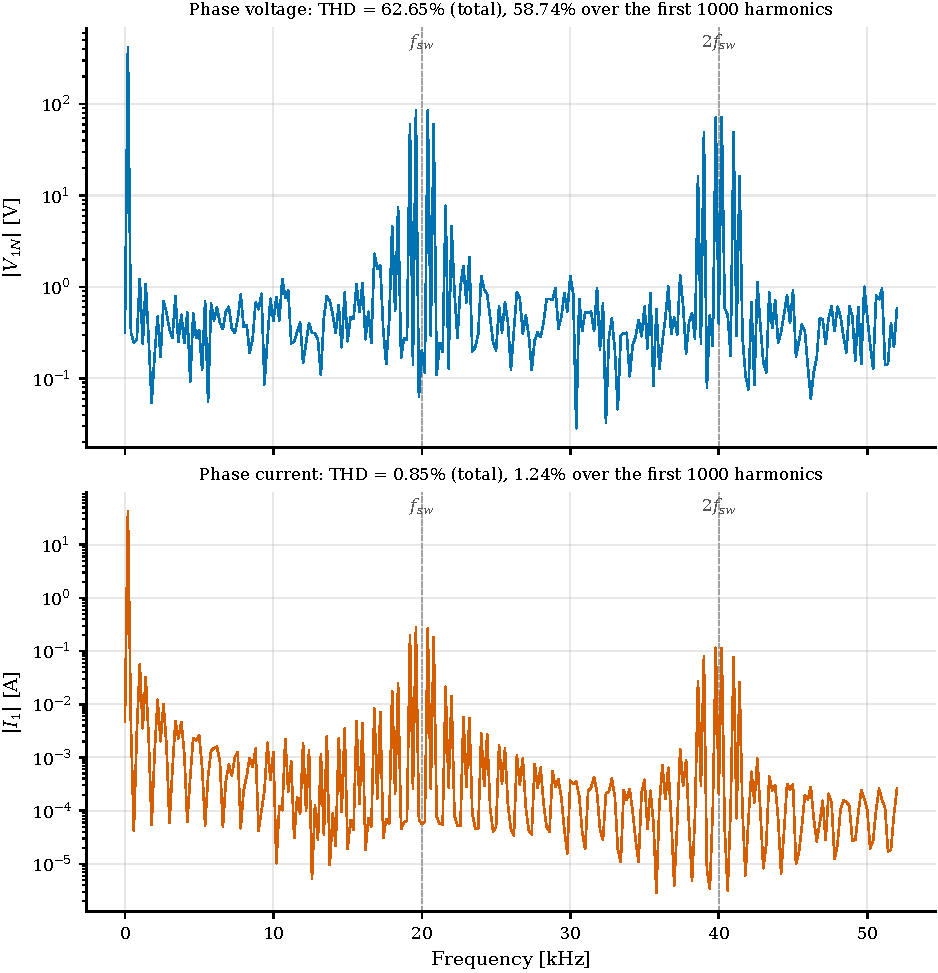
\includegraphics[width=\textwidth]{plecs_07_spettri_fft.pdf}
\caption{Spectra of the phase voltage $v_{1N}$ and of the phase current
$i_1$. The sidebands around \SI{20}{\kilo\hertz} and its multiples are clear
in the voltage. The load inductance attenuates them in the current.}
\label{fig:fft}
\end{figure}

The THD uses the RMS value of the waveform:
%
\begin{equation}
  \mathrm{THD} = \frac{\sqrt{V_\mathrm{rms}^2 - V_1^2}}{V_1} .
  \label{eq:thd}
\end{equation}
%
The phase voltage has a THD of \SI{62.6}{\percent}. A sum truncated at 50
harmonics reaches only \SI{10}{\kilo\hertz}, misses the switching spectrum
and gives about \SI{1}{\percent}. The current THD is \SI{0.85}{\percent}:
the load inductance filters the voltage harmonics.

\section{Check of the vendor loss tables}
\label{sec:losstables}

The losses of \cref{ch:losses} come from the vendor tables, so the tables
are checked against the datasheet. The vendor library has the same device in
two folders: a pair of files (\texttt{MOSFET} and \texttt{Diode}) and a
single file of class \texttt{MOSFET with Diode}. The datasheet gives two
switching energies at the test point (\SI{800}{\volt}, \SI{80.28}{\ampere},
\SI{175}{\celsius}, \SI{2.5}{\ohm}):
\begin{itemize}
  \item free-wheeling through an external SiC diode: $\Eon = \SI{1287}{\micro\joule}$;
  \item free-wheeling through the body diode: $\Eon = \SI{2552}{\micro\joule}$.
\end{itemize}
This design has no external diode, so only the second case applies.
\Cref{tab:losstable-check} compares the table entries with both cases.

\begin{table}[htbp]
\centering
\caption{Vendor table entries against the two datasheet
cases~\cite{wolfspeed_e3m0016,wolfspeed_plecs}.}
\label{tab:losstable-check}
\zebra
\begin{tabular}{lrrrl}
\toprule
Quantity & XML table & SiC diode & Body diode & Matches \\
\midrule
$\Eon$  & \SI{2545.8}{\micro\joule} & \SI{1287}{\micro\joule} & \SI{2552}{\micro\joule} & body diode \\
$\Eoff$ & \SI{784.7}{\micro\joule}  & \SI{805}{\micro\joule}  & \SI{788}{\micro\joule}  & body diode \\
\bottomrule
\end{tabular}
\end{table}

The tables match the body-diode case within \SI{0.24}{\percent} on $\Eon$
and \SI{0.41}{\percent} on $\Eoff$. The name \texttt{MOSFET with Diode}
means a MOSFET modelled together with its own body diode. The tables can
therefore be used without correction.

\section{Validation against the formulas}
\label{sec:validation}

Four checks compare the model with the analytical results.

\subsection{DC-link capacitor current}

The model is run at exactly \SI{30}{\Arms} for eight power factors, with
the modulation amplitude of \SI{427}{\volt}. \Cref{tab:ic-check} compares
the capacitor current with \cref{eq:icrms}.

\begin{table}[htbp]
\centering
\caption{DC-link capacitor RMS current at \SI{30}{\Arms}: simulation and
\cref{eq:icrms}.}
\label{tab:ic-check}
\zebra
\begin{tabular}{rrrr}
\toprule
$\cos\varphi$ & Simulated [\si{\ampere}] & Formula [\si{\ampere}] & Difference \\
\midrule
0.02 & 16.28 & 16.28 & \SI{0.0}{\percent} \\
0.10 & 16.25 & 16.24 & \SI{0.1}{\percent} \\
0.30 & 16.01 & 16.01 & \SI{0.0}{\percent} \\
0.50 & 15.56 & 15.53 & \SI{0.2}{\percent} \\
0.70 & 14.89 & 14.79 & \SI{0.7}{\percent} \\
0.87 & 14.15 & 13.91 & \SI{1.7}{\percent} \\
0.95 & 13.74 & 13.40 & \SI{2.5}{\percent} \\
1.00 & 14.47 & 12.67 & \SI{14}{\percent} \\
\bottomrule
\end{tabular}
\end{table}

The agreement is within \SI{2.5}{\percent} up to $\cos\varphi = 0.95$. At
$\cos\varphi = 1$ the difference is larger. The load at this point has only
\SI{0.1}{\milli\henry}, so the output current has a large ripple. The
formula of the course assumes a negligible ripple.

At the worst case of \cref{sec:dclink} ($\cos\varphi = 1$, $M_f = 0.306$) the
formula gives \SI{19.49}{\ampere}. The model with the \SI{5}{\micro\henry}
source gives about \SI{19.9}{\ampere}.

\subsection{Switching loss against frequency}

The switching loss must be linear in $\fsw$ and zero at $\fsw = 0$. A sweep
from \SI{10}{} to \SI{30}{\kilo\hertz} gives \SI{596.5}{\micro\joule} per
device and per cycle, with $R^2 = \num{1.0000}$ and an intercept of
\SI{-1.01}{\watt}.

\subsection{Conduction loss}

The conduction loss was recomputed in Python. The script integrates the
vendor voltage-drop tables over a sinusoidal current of \SI{30.006}{\Arms},
at the junction temperature of the thermal loop, \SI{81.84}{\celsius}:
\begin{itemize}
  \item channels: \SI{54.56}{\watt};
  \item extra loss in the dead time (\cref{eq:deadtime-loss}): \SI{3.21}{\watt};
  \item total: \SI{57.77}{\watt}, against \SI{57.64}{\watt} from PLECS
        (\SI{0.23}{\percent}).
\end{itemize}
The same tables are used in \cref{ch:thermal,ch:losses} for the estimates
made outside PLECS.

\subsection{Steady-state analysis of PLECS}

The thermal results of this report come from time-domain runs. The case
temperature is iterated until losses and temperature agree. PLECS also has a
steady-state analysis, as the brief suggests. It finds the periodic solution
directly and is a second method. The period to give is $1/f_\mathrm{ref}$,
the period of the output, not $1/\fsw$. With $1/\fsw$ the analysis returned
\SI{2}{\watt} of total loss.

With the correct period, the final model gives:
\begin{itemize}
  \item steady-state analysis: \SI{128.52}{\watt} and $\Tj = \SI{81.89}{\celsius}$;
  \item time-domain method: \SI{128.09}{\watt} and $\Tj = \SI{81.84}{\celsius}$.
\end{itemize}
The difference is \SI{0.33}{\percent} on the loss and \SI{0.05}{\celsius}
on the junction. Over the whole sweep of $\Rthcs$ of \cref{ch:thermal}, from
\SI{0.2}{} to \SI{1.2}{\celsius\per\watt}, the two methods agree within
\SI{0.35}{\percent} and \SI{0.12}{\celsius}.

The steady-state analysis has one limit. It uses one case resistance shared
by the six devices, which is correct at the rated point because their losses
are equal. At locked rotor it gives \SI{90.6}{\celsius} for the hottest
junction, against \SI{111.1}{\celsius} with one resistance per device
(\cref{sec:lockedrotor}). Locked rotor therefore uses the per-device method.

\section{DC-link ripple}

\begin{figure}[htbp]
\centering
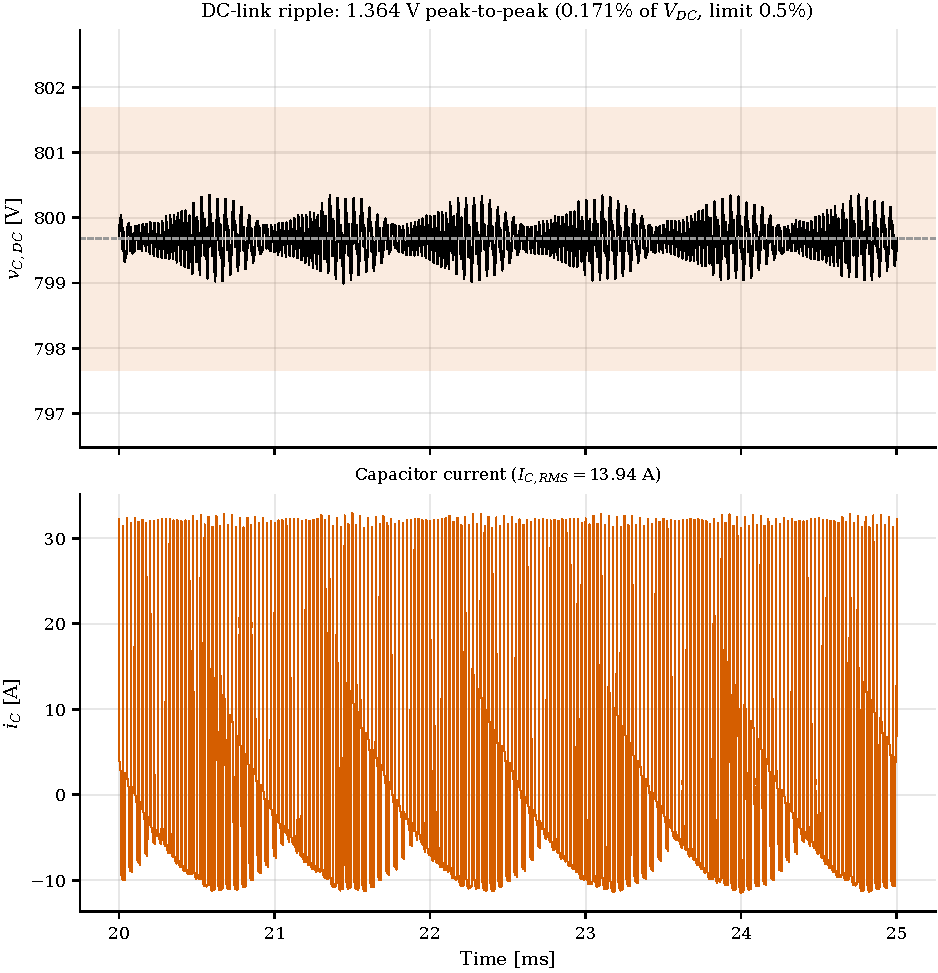
\includegraphics[width=\textwidth]{plecs_04_ripple_dc_link.pdf}
\caption{DC-link voltage ripple at the rated point, with the
\SI{5}{\micro\henry} source inductance: \SI{1.36}{\volt} peak-to-peak on
\SI{800}{\volt}, that is \SI{0.17}{\percent}, against the
\SI{0.5}{\percent} limit.}
\label{fig:ripple}
\end{figure}

The ripple at the rated point is \SI{1.36}{\volt}. Over the whole operating
range the worst case is \SI{2.86}{\volt}, inside the \SI{4}{\volt} limit
(\cref{sec:dclink}). The model with an ideal voltage source instead of the
\SI{5}{\micro\henry} cables would give \SI{0.43}{\volt}: the ideal source
absorbs part of the ripple current, so the cable inductance must be kept in
the model.
